
% Preamble
\documentclass[12pt]{article}

% Packages
\usepackage{amsmath}
\usepackage{graphicx}
% Document
\begin{document}


\section*{Self-Attention Mechanism Calculation}

Given the input sequence
\[
X = \begin{bmatrix}
0.8 & -0.4 \\
1.2 & 0.3 \\
-0.5 & 1.1 \\
\end{bmatrix}
\]
and learnable weight matrices
\[
W_Q = \begin{bmatrix}
0.6 & -0.2 \\
0.1 & 0.5
\end{bmatrix}, \quad
W_K = \begin{bmatrix}
-0.3 & 0.7 \\
0.4 & 0.9
\end{bmatrix}, \quad
W_V = \begin{bmatrix}
1.0 & -0.5 \\
0.2 & 0.8
\end{bmatrix}.
\]


\[
Q = X W_Q,\quad K = X W_K, \quad V = X W_V
\]

\[
Q = \begin{bmatrix}
0.44 & -0.36 \\
0.75 & -0.09 \\
        -0.19 & 0.65
\end{bmatrix}
K = \begin{bmatrix}
-0.4 & 0.20 \\
-0.24 & 1.11 \\
0.59 & 0.64 \\
\end{bmatrix}
V = \begin{bmatrix}
0.72 & -0.72 \\
1.26 & -0.36 \\
-0.28 & 1.13 \\
\end{bmatrix}
\]

\[
QK^T =
\begin{bmatrix}
-0.2480 & -0.5052 & 0.0292 \\
-0.3180 & -0.2799 & 0.3849 \\
0.2060 & 0.7671 & 0.3039
\end{bmatrix}
\]

\[
\text{Softmax}(z_i) = \frac{e^{z_i}}{\sum_{j} e^{z_j}}
\]

\[
\text{Softmax\_Scores} =
\begin{bmatrix}
0.3233 & 0.2500 & 0.4266 \\
0.2464 & 0.2560 & 0.4976 \\
0.2594 & 0.4546 & 0.2861
\end{bmatrix}
\]
\]

\[
\text{attention scores}=
\begin{bmatrix}
0.4284 & 0.1593 \\
0.3606 & 0.2928 \\
0.6794 & -0.0272
\end{bmatrix}
\]
\newpage



\begin{figure}
    \centering
    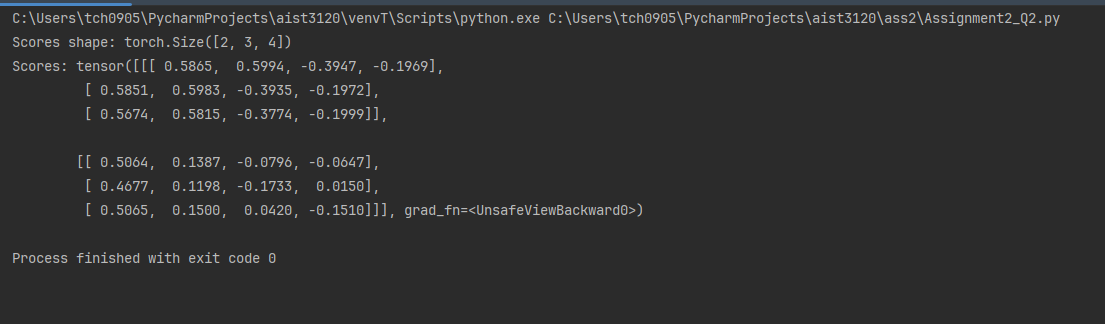
\includegraphics[width=1\linewidth]{2.png}
    \caption{Enter Caption}
    \label{fig:enter-label}
\end{figure}
\end{document}